\subsection{Analysis by Size}
\label{analysis by size}
We have presented the respondents' company size in Figure \ref{fig:company size}. It seems that our survey respondents are mainly from medium and small companies.

\begin{figure}[h]
\centering
  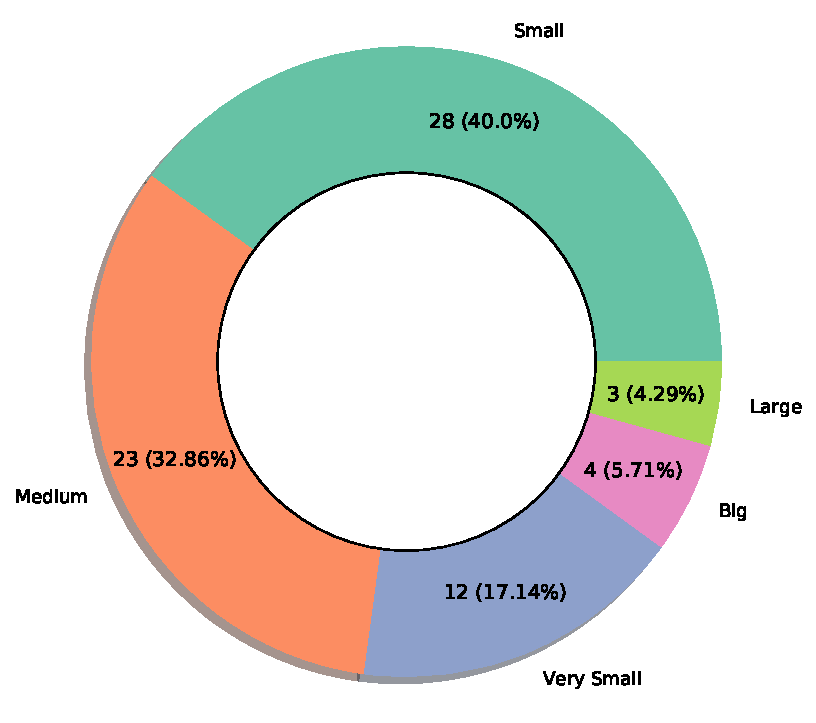
\includegraphics[scale=0.45]{Figures/Company_Size}
  \caption{Distribution of the size of respondents companies}
  \label{fig:company size}
\end{figure}

To get an idea of the companies' distribution of experience, we plotted the experience along with company size in Figure \ref{fig:experience and company size}. It is expected that companies will have a composition of different experience levels. However, we observe that big and large companies do not pose any composition of different experience levels. It is often seen that the senior position of big and large companies are often held by international candidates rather than a local candidate. However, we have too few respondents from big and large companies to draw any conclusion.

\begin{figure}[h]
\centering
  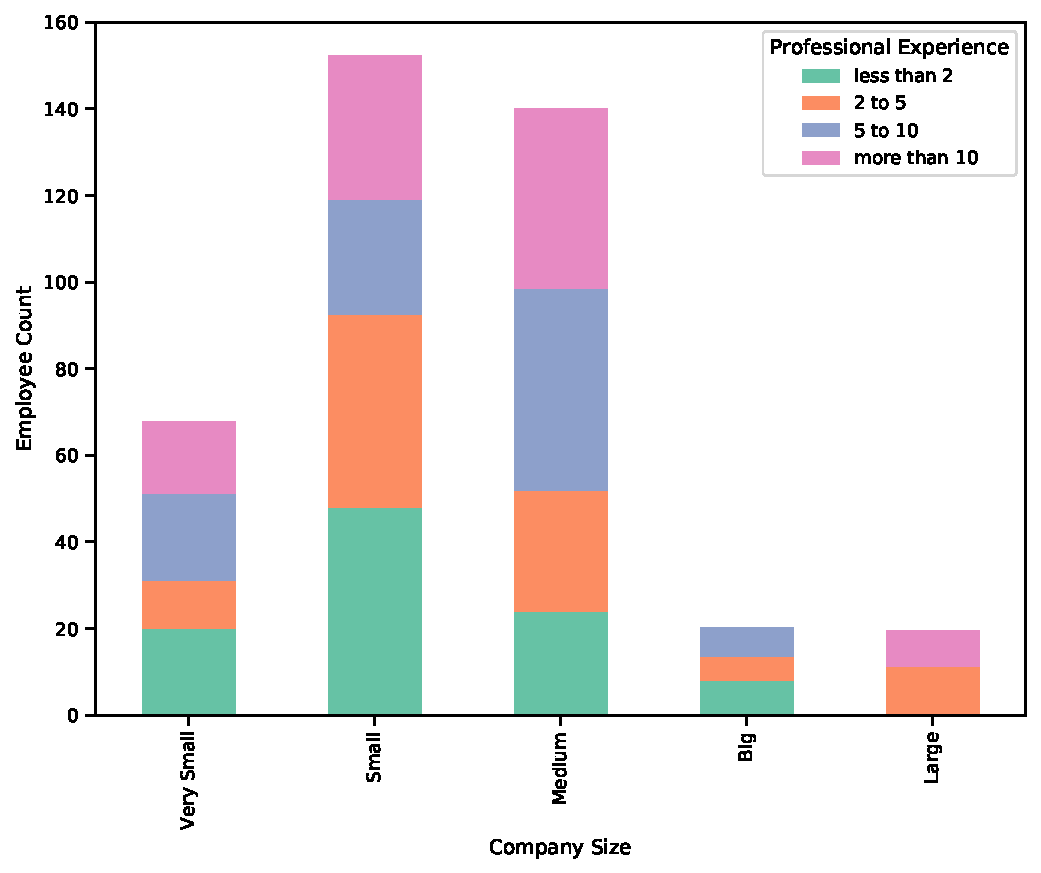
\includegraphics[scale=0.45]{Figures/Employee_Company_Size}
  \caption{Distribution of the experience}
  \label{fig:experience and company size}
\end{figure}

Testing practices are considered to be related to company culture, and it is believed large companies maintain better company culture than small companies. To check automatic testing practices among large and small companies, we plotted them together in Figure \ref{fig:auto tets level and company size}. It is clear from the Figure \ref{fig:auto tets level and company size} that the highest level of automatic testing is mostly done in medium-sized companies.

\begin{figure}[h]
\centering
  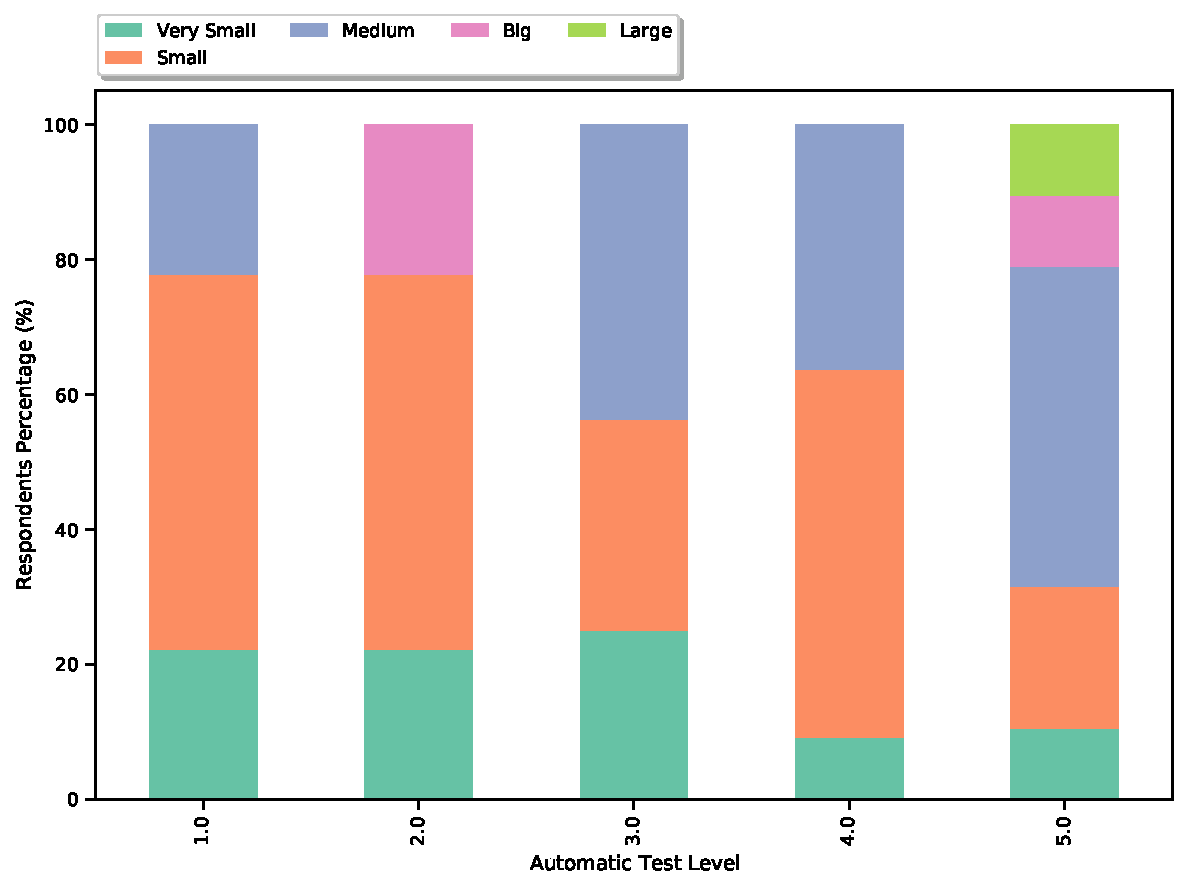
\includegraphics[scale=0.45]{Figures/Auto_Test_Company_Size.pdf}
  \caption{Automatic test level vs company size}
  \label{fig:auto tets level and company size}
\end{figure}

To understand how the technology stack is distributed among companies, we plotted the technology stack with company size in Figure \ref{fig:technology and company size}. It is clear from Figure \ref{fig:technology and company size} that comparatively newer technology is prevalent only in small and very small companies. One reason for such distribution can be that to survive in the competitive market, small and very small companies invested their time in newer technologies that are less practiced/ignored by large companies.

\begin{figure}[h]
\centering
  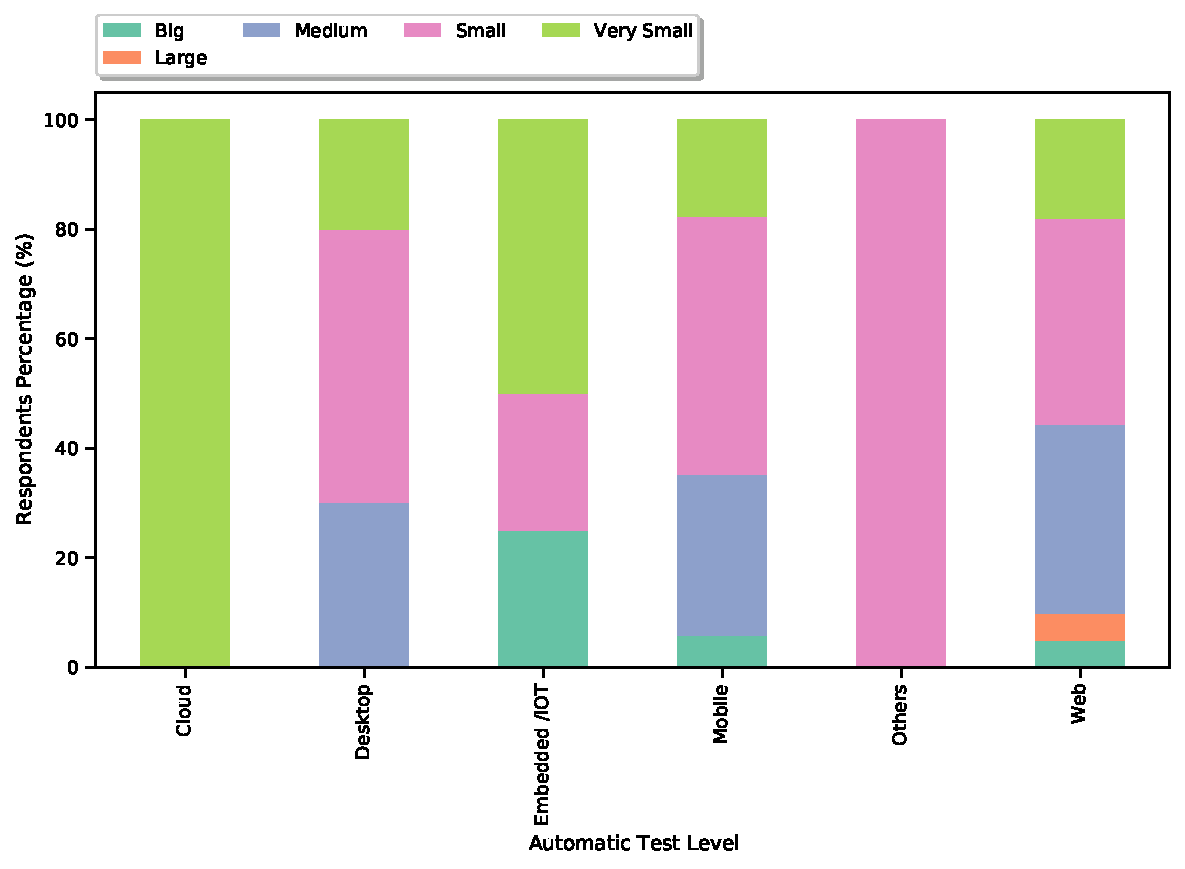
\includegraphics[scale=0.45]{Figures/Technology_Company_Size}
  \caption{Technology stack of companies}
  \label{fig:technology and company size}
\end{figure}